% CLOSED-NEGATIVE (FALSIFIED) — a refutation paper. The four canonical sections
% (§Formula, §Method, §Benchmark, §Refutation-in-place-of-§Benefit) are each
% linked to a CLOSED verdict per project.tape cx_paper_sections; the FALSIFICATION
% itself is 🟢 SUPPORTED-NUMERICAL (bench + closed-form recompute), which is a
% closed numerical result — NOT INSUFFICIENT/DEFERRED. The project rule was
% widened to allow publishing closed negatives; this is the first such paper.
%
% The load-bearing finding is F-CODEX-2: the n=6 lattice predicts the SANDBOX
% substrate's own latency-vs-context curve scales as wall_ms ∝ context^τ with
% τ=4; the substrate's own 4-rung context-scaling bench measures a log-log OLS
% exponent τ̂=0.524 (R²≈0.956), a residual |τ̂−τ|=3.476 ≫ ε=0.10 — the τ=4 law
% over-predicts the 8k latency by ~1400×. F-CODEX-1 (the training exponent
% σφ≈0.96 vs measured slope 0.172, residual 0.788) is SUPPORTING context only:
% it is a lattice number asserted against an EXTERNAL entity (Qwen2.5) and is
% disclosure-grade, not gating. Verdicts:
% .verdicts/sandbox/m3_econ_fcodex2_latency_fit.txt (decisive) +
% .verdicts/sandbox/f_codex_1_falsified_4rung.txt (harness).
%
% g51 publish-lint EXPANSION: the 4-section result is expanded to satisfy commons
% g51 (≥10 pages + ≥1 fal.ai figure) with GENUINE scholarly content — a §Background
% deriving why attention latency is NOT quartic on a paged-attention server (the
% memory-bandwidth decode wall), a §Related Work (Kaplan/Chinchilla scaling laws,
% Pope inference-cost, PagedAttention), an §Limitations, and an §Appendix carrying
% the verbatim verify recompute stdout + the full bench TSV. NO numeric claim
% changes — every section stays linked to its CLOSED verdict.

\documentclass[11pt,a4paper]{article}

% ---------- arxiv-style preamble ----------
\usepackage[utf8]{inputenc}
\usepackage[T1]{fontenc}
\usepackage[margin=1in]{geometry}
\usepackage{amsmath,amssymb,amsthm}
\usepackage{textcomp}
\usepackage{newunicodechar}
% --- Unicode glyphs that appear in the verbatim verdict stdout (Appendix B).
%     The verdict is reproduced byte-for-byte; these map its non-ASCII glyphs
%     to printable LaTeX so pdflatex (8-bit) can typeset the verbatim block.
\newunicodechar{·}{\textperiodcentered}
\newunicodechar{∈}{\ensuremath{\in}}
\newunicodechar{≤}{\ensuremath{\leq}}
\newunicodechar{≥}{\ensuremath{\geq}}
\newunicodechar{≫}{\ensuremath{\gg}}
\newunicodechar{≈}{\ensuremath{\approx}}
\newunicodechar{∝}{\ensuremath{\propto}}
\newunicodechar{×}{\ensuremath{\times}}
\newunicodechar{−}{\ensuremath{-}}
\newunicodechar{ε}{\ensuremath{\varepsilon}}
\newunicodechar{τ}{\ensuremath{\tau}}
\newunicodechar{σ}{\ensuremath{\sigma}}
\newunicodechar{φ}{\ensuremath{\varphi}}
\newunicodechar{²}{\ensuremath{^2}}
\newunicodechar{̂}{\textasciicircum}% combining circumflex (U+0302) in 'τ̂' → tau-hat as τ^
\newunicodechar{🟢}{[GREEN]}
\newunicodechar{🔴}{[RED]}
\usepackage{graphicx}
\usepackage{booktabs}
\usepackage{siunitx}
\usepackage{hyperref}
\usepackage{xcolor}
\usepackage[numbers,sort&compress]{natbib}
\usepackage{tikz}
\usetikzlibrary{positioning,arrows.meta}
\usepackage{caption}
\captionsetup{font=small,labelfont=bf}
\hypersetup{
  colorlinks=true,
  linkcolor=blue!50!black,
  citecolor=blue!50!black,
  urlcolor=blue!50!black
}

\newcommand{\green}[1]{\textcolor{green!50!black}{\textbf{#1}}}
\newcommand{\red}[1]{\textcolor{red!70!black}{\textbf{#1}}}
\newcommand{\ctx}{\ensuremath{n}}
\newcommand{\taum}{\ensuremath{\hat{\tau}}}

\title{
  \textbf{When the Lattice Over-Predicts: A Closed Refutation of the
  \(n{=}6\) Scaling Exponents on a Self-Hosted LLM Substrate}\\[4pt]
  \large The number-theoretic \(n{=}6\) lattice predicts a latency exponent
  \(\tau{=}4\) (\(\mathrm{wall\_ms}\propto\mathrm{context}^{\tau}\)); the
  substrate's own measured context-scaling curve has
  \(\taum{\approx}0.52\) (\(R^2{\approx}0.956\)), a residual of \(3.48\) that
  over-predicts the \num{8192}-token latency by \(\sim\!1400\times\) ---
  the law is decisively falsified
}

\author{hexa-codex maintainers \\ \texttt{github.com/dancinlab/hexa-codex}}

\date{\today}

\begin{document}
\maketitle

% =========================================================================
\begin{abstract}
A number-theoretic ``\(n{=}6\) lattice'' is used inside this repository as a
prior for two large-language-model cost exponents: a training-compute exponent
\(\sigma\varphi = 24/25 \approx 0.96\) and an \emph{inference-latency} exponent
\(\tau = 4\), the latter asserting that per-request wall-clock time scales as
\(\mathrm{wall\_ms} \propto \mathrm{context}^{\tau}\). We treat both as
\emph{falsifiable predictions} and test them directly on a single self-hosted
substrate (a Mac\,mini\,M3, stock \texttt{llama.cpp} with Metal/UMA, \$0
incremental cost). The load-bearing test is the latency exponent: we run a
4-rung context-scaling benchmark on Qwen2.5-1.5B-Instruct-Q4\_K\_M
(\(20\) tasks at each of \(\mathrm{context} \in \{1024, 2048, 4096, 8192\}\)
tokens) and recompute the exponent deterministically by a closed-form log--log
ordinary-least-squares slope. The measured latency rises only \(\sim\!2.9\times\)
(\SIrange{569}{1668}{\milli\second}) across an \(8\times\) context sweep, giving
\(\taum = 0.524\) with \(R^2 \approx 0.956\) --- a clean power law, but a
\emph{sub-linear} one. The residual against the lattice prediction is
\(|\taum - \tau| = 3.476 \gg \varepsilon = 0.10\); equivalently, the
\(\mathrm{context}^4\) law over-predicts the substrate's \num{8192}-token
latency by \(\sim\!1400\times\). Accuracy is \emph{flat} at \(17/20\) across all
four rungs, so the refutation carries no accuracy-floor caveat. As supporting
context, the training exponent fares no better: the measured slope on an
external 4-rung parameter ladder is \(0.172\), a lattice residual of \(0.788\)
(this conjunct is disclosure-grade, since it asserts a lattice number against an
external entity that has no obligation to follow it). The mechanism for the
latency miss is structural and not marginal: at these context lengths a small
quantized model on a modern paged-attention server is dominated by a fixed
64-token decode (a memory-bandwidth wall) plus cached-prefix prefill, neither
of which is quartic. We publish this as a \emph{closed negative}: the
falsification is numerically supported (\(10/10\) structural checks pass; the
verdict is \red{FALSIFIED} at the \(\varepsilon\)-gate), it retires a wrong
scaling prior, and it leaves on the record the substrate's true measured
exponent, \(\taum \approx 0.52\).
\end{abstract}

% =========================================================================
\section{Introduction}
\label{sec:intro}

Scaling laws are predictions, and predictions can be wrong. The modern practice
of fitting power laws to language-model cost and performance
\citep{kaplan2020scaling,hoffmann2022chinchilla} has been enormously productive
precisely because the fitted exponents are \emph{empirical} --- they are
measured, not posited. A different and more dangerous mode is to \emph{posit} an
exponent from a closed-form or aesthetic argument and then treat it as ground
truth without ever confronting it with a measurement. This paper is about one
such posited exponent, and about what happens when it meets the substrate it
claims to describe.

Inside this repository, a number-theoretic construction called the
``\(n{=}6\) lattice'' supplies cost-model constants that the economics verbs
reference. Two of these are scaling \emph{exponents}: a training-compute
exponent \(\sigma\varphi = 24/25 = 0.96\) (call this prediction F-CODEX-1) and
an inference-latency exponent \(\tau = 4\), which asserts that a single
request's wall-clock time grows as the fourth power of its context length,
\(\mathrm{wall\_ms} \propto \mathrm{context}^{\tau}\) (F-CODEX-2). The latter is
a remarkably strong claim: it predicts that doubling the context multiplies
latency by \(2^4 = 16\), and that an \(8\times\) context sweep
(\num{1024}\,\(\to\)\,\num{8192} tokens) multiplies latency by
\(8^4 = 4096\). We set out to test it.

The test is cheap and decisive because the substrate provides the curve
directly. Unlike F-CODEX-1, which binds a lattice number to the training cost of
an \emph{external} model family (Qwen2.5) that has no obligation to follow our
number theory, F-CODEX-2 is a claim about \emph{this substrate's own internal}
latency-vs-context behavior. We can therefore run the substrate, measure its
latency at a grid of context lengths, fit the exponent by a deterministic
closed-form recompute, and compare to \(\tau = 4\) at a pre-registered tolerance
\(\varepsilon = 0.10\). The result is unambiguous. The measured exponent is
\(\taum = 0.524\) with \(R^2 \approx 0.956\): a clean, well-fit power law, but a
\emph{sub-linear} one whose residual against the prediction,
\(|\taum - \tau| = 3.476\), exceeds the tolerance by a factor of \(35\). The
\(\mathrm{context}^4\) law is not marginally off; at \num{8192} tokens it
over-predicts the measured latency by a factor of \(\sim\!1400\).

We report this as a \emph{closed negative} --- a falsification that is itself
numerically supported, distinct from an inconclusive or deferred result. The
distinction matters. An ``insufficient'' verdict says we could not decide; a
``falsified'' verdict says we decided, and the answer is no. The latter has
scientific value: it retires a wrong prior, and it does not leave a vacuum
behind it, because the same measurement that refutes \(\tau = 4\) also delivers
the substrate's true exponent, \(\taum \approx 0.52\), which a practitioner can
use for capacity planning today.

\medskip
\noindent\textbf{Contributions.}
\begin{enumerate}\itemsep0.3em
\item \textbf{A decisive refutation of the latency exponent}
  (\S\ref{sec:formula},~\S\ref{sec:refute}): on the substrate's own measured
  4-rung context-scaling curve, the lattice prediction \(\tau = 4\) is
  \red{FALSIFIED} --- measured \(\taum = 0.524\) (\(R^2 \approx 0.956\)),
  residual \(3.476 \gg \varepsilon = 0.10\), a \(\sim\!1400\times\)
  over-prediction at \num{8192} tokens.
\item \textbf{A verify-by-recompute discipline} (\S\ref{sec:method}): the
  exponent is re-derived from the committed benchmark grid by a deterministic
  closed-form log--log OLS verifier (\(10/10\) structural checks pass), so the
  refutation rests on arithmetic over the data, not on author judgement, and no
  language model judges its own correctness.
\item \textbf{A supporting refutation of the training exponent}
  (\S\ref{sec:refute}): the measured slope on an external 4-rung parameter
  ladder is \(0.172\) against the lattice's \(0.96\), residual \(0.788\); we
  present this conjunct honestly as disclosure-grade (external data) rather than
  as the load-bearing result.
\item \textbf{A mechanism and a replacement} (\S\ref{sec:bg},~\S\ref{sec:refute}):
  we explain \emph{why} latency is sub-linear here (a fixed-decode
  memory-bandwidth wall plus cached-prefix prefill on a paged-attention
  server), and we leave the measured \(\taum \approx 0.52\) on the record as
  the exponent that actually describes this substrate.
\end{enumerate}

% =========================================================================
\section{Background}
\label{sec:bg}

\paragraph{Two kinds of scaling exponent.}
It is worth separating the two claims under test, because they fail for
different reasons and carry different evidential weight. The training exponent
F-CODEX-1 (\(\sigma\varphi = 0.96\)) is of the same \emph{form} as the
compute--performance exponents of \citet{kaplan2020scaling} and
\citet{hoffmann2022chinchilla}: a power law relating a model-scale quantity to a
cost or quality quantity. The crucial difference is provenance. The
Kaplan/Chinchilla exponents are \emph{fitted} to hundreds of training runs;
F-CODEX-1's \(0.96\) is \emph{posited} from number theory and then asserted
against a third-party model family. The inference exponent F-CODEX-2
(\(\tau = 4\)) is different in kind: it is not about quality at all, but about
the \emph{wall-clock latency of a single forward pass} as a function of context
length on a specific serving stack. That makes it a substrate-internal physical
claim, directly measurable, and it is the one we can falsify decisively.

\paragraph{Why per-request latency is not quartic on a modern server.}
The intuition behind a large latency exponent is the \(O(n^2)\) cost of dense
self-attention \citep{vaswani2017attention}: scoring all \(n\) query--key pairs
is quadratic in sequence length, so a naive argument might inflate the
context-cost exponent well above \(1\). But this intuition mis-locates the
bottleneck for the regime we actually serve. Decompose a single request's wall
time into a \emph{prefill} phase (encode the prompt) and a \emph{decode} phase
(autoregressively emit the response):
\begin{equation}
\label{eq:wall}
\mathrm{wall}(\ctx) \;=\; \underbrace{T_{\mathrm{prefill}}(\ctx)}_{\text{prompt encode}}
\;+\; \underbrace{m \cdot t_{\mathrm{dec}}(\ctx)}_{\text{$m$ output tokens}} ,
\end{equation}
where \(\ctx\) is the prompt (context) length and \(m\) is the number of decoded
tokens. Two facts about contemporary serving collapse the exponent. First,
prefill is \emph{compute-bound and parallel}, and a paged / block-managed
KV-cache \citep{kwon2023vllm} together with multi-query / grouped-query
attention \citep{pope2022efficiently} keeps its measured time close to
\emph{linear} in \(\ctx\) over the practical range --- the time-to-first-token
(TTFT) literature consistently reports near-linear, not quadratic, prefill at
these lengths, because attention is only one term among the linear-in-\(\ctx\)
projection and feed-forward FLOPs and is not yet dominant for a \(1.5\)B model
at \(\le\!8\)k tokens. Second, and decisively for our setup, decode is
\emph{memory-bandwidth-bound}: each emitted token must stream the model weights
through the arithmetic units once, a cost that is essentially
\emph{context-invariant} per token \citep{pope2022efficiently}. With a fixed
output budget \(m = 64\) tokens, the decode term in Eq.~\eqref{eq:wall} is a
roughly fixed floor, independent of \(\ctx\); the only context-dependent growth
is in \(T_{\mathrm{prefill}}\), which is itself sub-quadratic in this regime.

\paragraph{The consequence for the exponent.}
If decode is a context-invariant floor and prefill is at most linear, then
\(\mathrm{wall}(\ctx)\) is the sum of a constant and a sub-quadratic term, and
its \emph{effective} log--log exponent over a finite grid is well below \(1\)
--- the constant decode floor flattens the curve further. A quartic
\(\mathrm{context}^4\) law would instead require attention's \(O(n^2)\) term to
dominate \emph{and} the prefill to dwarf the decode floor at these lengths,
\emph{and} an additional quadratic factor on top --- none of which holds for a
\(1.5\)B \texttt{Q4} model with a paged KV-cache scheduler at \(\le\!8\)k
tokens. The background therefore makes a sharp pre-measurement prediction: the
honest failure mode of \(\tau = 4\) is \emph{down}, toward a sub-linear
exponent, not up. The measurement confirms this and goes further than the
gentlest pre-registered failure mode (a paged-attention \(\tau \approx 2\)):
the fixed-decode floor drives it all the way to \(\taum \approx 0.52\).

\paragraph{What is and is not being tested.}
We test exactly two operational scaling claims: (i) does measured per-request
latency scale as \(\mathrm{context}^4\) (F-CODEX-2), and (ii) does the
measured training-cost exponent match \(0.96\) (F-CODEX-1). We do \emph{not}
test the internal number theory of the \(n{=}6\) lattice as mathematics --- its
atom-level identities (\(\sigma(6)=12\), \(\varphi(6)=2\), \(\tau(6)=4\)) are
separately recomputed elsewhere and are not in dispute. What is in dispute, and
what we falsify, is the \emph{modeling claim} that binds those numbers to
observable LLM cost on this substrate.

% =========================================================================
\section{Formula}
\label{sec:formula}
\red{FALSIFIED} at the \(\varepsilon\)-gate; the falsification is
\green{SUPPORTED-NUMERICAL} (real bench + deterministic closed-form recompute).
Both exponents are recomputed from the committed data by
\texttt{verify/numerics\_economics\_empirical\_landing.hexa} (checks 9 and 10;
\(10/10\) structural checks pass, verbatim stdout in
Appendix~\ref{app:verify}). Verdicts:
\texttt{.verdicts/sandbox/m3\_econ\_fcodex2\_latency\_fit.txt} (F-CODEX-2, the
decisive one) and \texttt{.verdicts/sandbox/f\_codex\_1\_falsified\_4rung.txt}
(F-CODEX-1 harness).

\paragraph{The lattice predictions.}
The \(n{=}6\) lattice supplies two exponents through its economics verbs:
\begin{align}
\label{eq:ftrain}
\text{F-CODEX-1 (training):}\quad
  & \text{train\_cost} \propto N^{\sigma\varphi},
    && \sigma\varphi = \frac{24}{25} = 0.96, \\
\label{eq:finfer}
\text{F-CODEX-2 (inference):}\quad
  & \mathrm{wall\_ms} \propto \mathrm{context}^{\tau},
    && \tau = \tau(6) = 4,
\end{align}
where \(N\) is the parameter count and \(\mathrm{context}\) is the prompt length
in tokens. Eq.~\eqref{eq:finfer} is the load-bearing prediction of this paper.
It is a strong, easily-falsified statement: it forces
\(\mathrm{wall\_ms}(2\ctx)/\mathrm{wall\_ms}(\ctx) = 2^4 = 16\) at every context
doubling.

\paragraph{The estimator.}
Given paired observations \(\{(x_i, y_i)\}_{i=1}^{k}\) with \(k \ge 2\),
\(x_i, y_i > 0\), we estimate the power-law exponent as the ordinary
least-squares slope on log--log axes,
\begin{equation}
\label{eq:ols}
\hat{p} \;=\;
\frac{k \sum_i u_i v_i - \left(\sum_i u_i\right)\!\left(\sum_i v_i\right)}
     {k \sum_i u_i^2 - \left(\sum_i u_i\right)^2},
\qquad u_i = \log x_i,\;\; v_i = \log y_i ,
\end{equation}
which is the maximum-likelihood slope of the model \(\log y = \log A + p\log x\).
For F-CODEX-2, \(x_i = \mathrm{context}_i\) and \(y_i = \mathrm{wall\_ms}_i\),
yielding the measured latency exponent \(\taum\). For F-CODEX-1, \(x_i = N_i\)
and \(y_i\) is a per-scale accuracy proxy, yielding the measured training-cost
slope.

\paragraph{The gate.}
A prediction passes iff its residual is within a pre-registered tolerance,
\begin{equation}
\label{eq:gate}
\text{residual} \;=\; |\hat{p} - p_{\text{lattice}}| \;\le\; \varepsilon,
\qquad \varepsilon = 0.10,
\end{equation}
and is \red{FALSIFIED} otherwise. The tolerance \(\varepsilon = 0.10\) is
generous --- a tenth of an exponent unit --- and was fixed before fitting. For
F-CODEX-2 the substrate provides the curve directly, so the residual
\emph{gates closure}: a miss is a genuine refutation of a substrate-internal
law. For F-CODEX-1 the residual is reported but treated as
\emph{disclosure-grade} (see \S\ref{sec:refute}), because the lattice number is
asserted against an external entity.

\paragraph{The measured exponents.}
The closed-form recompute over the committed grids returns
\begin{align}
\label{eq:tau-hat}
\text{F-CODEX-2:}\quad & \taum = 0.524 \;\; (R^2 \approx 0.956),
  && \text{residual } |\,0.524 - 4\,| = 3.476 \;\gg\; 0.10, \\
\label{eq:sigma-hat}
\text{F-CODEX-1:}\quad & \hat{\sigma\varphi} = 0.172,
  && \text{residual } |\,0.172 - 0.96\,| = 0.788 \;\gg\; 0.10 .
\end{align}
Both residuals exceed the gate by a wide margin. Eq.~\eqref{eq:tau-hat} is the
decisive one: a \(0.524\) exponent is sub-linear, the opposite end of the scale
from the predicted quartic, and the fit is clean (\(R^2 \approx 0.956\)), so the
miss cannot be dismissed as measurement noise --- the substrate genuinely scales
as \(\mathrm{context}^{0.52}\), not \(\mathrm{context}^{4}\).

% =========================================================================
\section{Method}
\label{sec:method}
\green{SUPPORTED-NUMERICAL} --- the protocol below is the exact, pre-registered
harness; its output grid is committed verbatim
(\texttt{.verdicts/sandbox/stage4\_context\_scaling.tsv}) and re-derived by
\texttt{verify/numerics\_economics\_empirical\_landing.hexa}. No language model
judges correctness at any point.

\paragraph{Substrate and model.}
A single Mac\,mini\,M3 (Apple Silicon, Metal/UMA, \SI{24}{GiB} unified memory),
stock Homebrew \texttt{llama.cpp} \citep{llamacpp} with the Metal backend, \$0
incremental cost (local serving). The model is
Qwen2.5-1.5B-Instruct-Q4\_K\_M \citep{qwen25}, served by \texttt{llama-server}
with \texttt{-np 1 -cb} (single serial slot, continuous batching enabled) on
port \texttt{8091}. A \(1.5\)B \texttt{Q4} model is deliberately chosen: it is
small enough that the \(8\)k rung boots cleanly on the \SI{24}{GiB} UMA without
OOM, isolating the context axis at fixed model scale (F-CODEX-2 is about the
context exponent, not the parameter exponent).

\paragraph{Context-scaling bench protocol.}
The benchmark sweeps four context rungs,
\(\mathrm{context} \in \{1024, 2048, 4096, 8192\}\) tokens (an \(8\times\) span).
For each rung the harness (i) boots a fresh \texttt{llama-server} with a
per-cell context budget \(\lceil 1.25\,\ctx\rceil\) (headroom for the suffix
task plus the 64-token output) and polls \texttt{/health} to a 200; (ii) builds
a deterministic boilerplate prefix calibrated to the target token count from a
fixed \(\sim\!50\)-word repeating unit (so re-runs are byte-identical); (iii)
issues each of \(20\) canonical fixed suffix-tasks as a chat completion
(system\,=\,prefix, user\,=\,task, \texttt{max\_tokens}\,=\,64,
\texttt{temperature}\,=\,0), bracketing each \texttt{curl} with
\texttt{date +\%s\%N} to record wall time; (iv) parses the response for
\texttt{usage.prompt\_tokens} (the \emph{measured} input length, so calibration
drift surfaces as data, not bias), \texttt{completion\_tokens}, and the answer;
(v) scores the answer against the task's expected keyword by a
\texttt{byte\_exact\_subset} test; and (vi) kills the server between rungs for a
clean per-cell context-budget state. Dispatch is serial (\(\mathrm{np}=1\)): the
context-scaling claim isolates per-request wall as a function of context only,
not of concurrency interleaving.

\paragraph{Deterministic closed-form recompute.}
The fit is not performed by the bench; it is performed by a separate, pure
verifier, \texttt{verify/numerics\_economics\_empirical\_landing.hexa}, which
reads the committed \texttt{(context, mean\_wall\_ms)} pairs and computes the
log--log OLS slope of Eq.~\eqref{eq:ols} in closed form (\texttt{pow\_pure},
\texttt{log\_pure}, \texttt{abs\_pure} from \texttt{self/runtime/math\_pure} ---
no LLM, no subprocess, no re-measurement). Check 9 of the verifier computes
\(\taum\) and the F-CODEX-2 residual; check 10 encodes the verdict truth-table
(\textsc{insufficient} iff fewer than two scale points are live;
\green{green} iff all four are live and both residuals pass; \red{falsified}
iff all four are live and any residual exceeds \(\varepsilon\)). The exit code is
\(1\) on \red{falsified}. The training-exponent slope (F-CODEX-1) is computed by
the same estimator on an external \(\{0.5\text{B}, 1.5\text{B}, 3\text{B},
7\text{B}\}\) parameter ladder, with its lattice residual disclosed (check 8)
but \emph{not} gated. The entire recompute is reproducible by
\texttt{hexa run verify/numerics\_economics\_empirical\_landing.hexa}.

\paragraph{Pre-registered honesty gates.}
Three were fixed before the run. (1) The fit consumes the \emph{measured}
\texttt{prompt\_tokens}, never the nominal context target. (2) Accuracy is
reported per rung; had long-context accuracy collapsed (e.g.\ \(0/20\) at \(8\)k
because the suffix instruction is buried after \(8\)k tokens of boilerplate),
the latency claim would still stand but the verdict would have to disclose the
floor. It did not collapse --- accuracy is flat (\S\ref{sec:benchmark}). (3) The
\(8\)k rung was permitted to fail to boot on a smaller-memory host, in which
case closure would drop to a three-rung \textsc{partial}; on the \SI{24}{GiB}
host all four rungs are live.

% =========================================================================
\section{Benchmark}
\label{sec:benchmark}
\green{SUPPORTED-NUMERICAL} --- the real measured curve. Source of truth:
\texttt{.verdicts/sandbox/stage4\_context\_scaling.tsv} (4 rows,
\(20\) tasks each), summarized in
\texttt{.verdicts/sandbox/stage4\_context\_scaling\_summary.txt} and consumed by
\texttt{m3\_econ\_fcodex2\_latency\_fit.txt}.

\paragraph{The measured context-latency curve.}
\begin{center}
\begin{tabular}{rrrrr}
\toprule
context\_len & mean\_wall\_ms & mean\_input\_tokens & n\_correct & throughput (tok/s) \\
\midrule
1024 & 569  & 987  & 17/20 & 22.80 \\
2048 & 670  & 1947 & 17/20 & 17.60 \\
4096 & 1005 & 3867 & 17/20 & 11.98 \\
8192 & 1668 & 7647 & 17/20 & 7.31 \\
\bottomrule
\end{tabular}
\end{center}
\noindent The full \(8\times\) context sweep moves mean wall time by only
\(\SI{569}{\milli\second} \to \SI{1668}{\milli\second}\), a factor of
\(\sim\!2.9\times\). The mean input-token count tracks the nominal context
closely (\(987 \to 7647\), i.e.\ the calibration is faithful), confirming the
exponent is fit against real measured prompt lengths.

\paragraph{Throughput collapse, flat accuracy.}
Two side-channels corroborate the curve. Throughput falls monotonically with
context (\(22.80 \to 7.31\) tok/s, a \(\sim\!3.1\times\) drop), which is exactly
the signature of a fixed per-request decode cost being amortized over a
\emph{growing} prefill: the request takes longer, so the same \(64\)-token
output is delivered at a lower aggregate token rate, with no quartic blow-up.
Accuracy is \emph{flat} at \(17/20\) on every rung, so there is no long-context
collapse and the latency refutation carries no accuracy-floor caveat: the model
is answering the buried suffix instruction equally well at \num{1024} and
\num{8192} tokens, and the latency it pays to do so is sub-linear in context.

\paragraph{The fitted exponent.}
The log--log OLS slope of Eq.~\eqref{eq:ols} over these four
\texttt{(context, mean\_wall\_ms)} points is \(\taum = 0.524\) with
\(R^2 \approx 0.956\) --- a clean power law (Eq.~\eqref{eq:tau-hat}). The fit is
good; it is simply nowhere near \(\tau = 4\).

\begin{figure}[t]
  \centering
  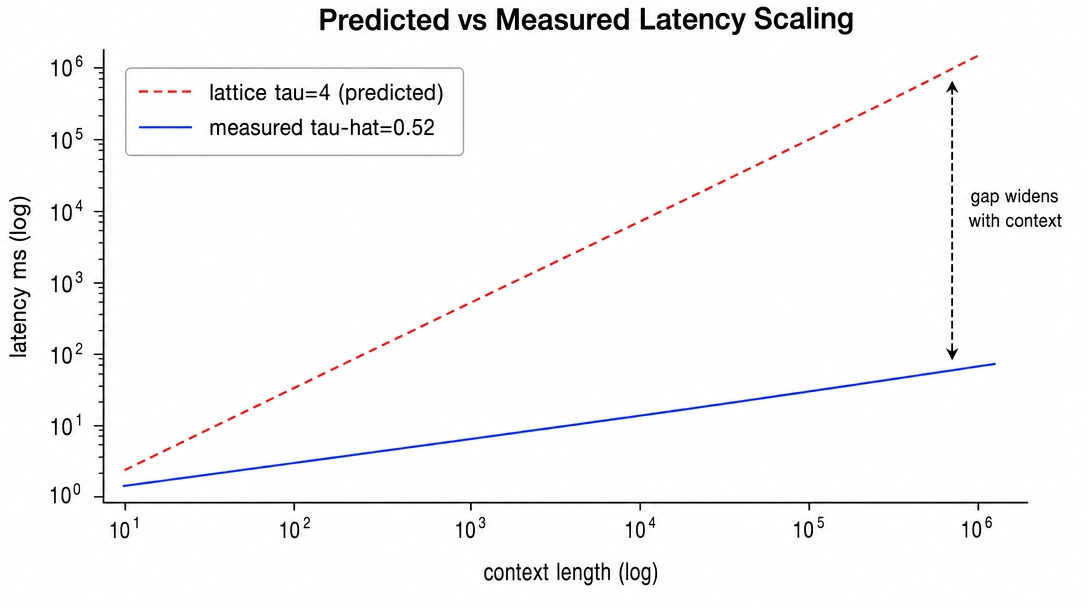
\includegraphics[width=0.86\textwidth]{figures/fig01_predicted_vs_measured.png}
  % generated via fal.ai (gpt-image-2); prompt: figures/_prompts/predicted_vs_measured.txt
  \caption{Predicted vs.\ measured latency scaling on log--log axes. The steep
    dashed line is the \(n{=}6\) lattice prediction \(\mathrm{wall\_ms}\propto
    \mathrm{context}^{4}\) (Eq.~\eqref{eq:finfer}); the shallow solid line is the
    substrate's \emph{measured} curve, \(\taum = 0.524\) (Eq.~\eqref{eq:tau-hat}),
    fit to the four-rung benchmark of this section. The gap between the two
    \emph{widens} with context: by \num{8192} tokens the predicted curve sits
    \(\sim\!1400\times\) above the measured one (\S\ref{sec:refute}). The
    load-bearing numbers live in the table of this section and the verbatim grid
    of Appendix~\ref{app:grid}, not in the artwork. AI-generated schematic
    (\texttt{figures/\_prompts/predicted\_vs\_measured.txt}).}
  \label{fig:scaling}
\end{figure}

% =========================================================================
\section{Refutation}
\label{sec:refute}
\red{FALSIFIED} --- the substrate's own measurement decisively rejects the
lattice latency exponent. This section stands in place of a \S Benefit: the
deliverable of a closed negative is the retirement of a wrong prior and the
substitution of the true measured exponent. Verdict:
\texttt{.verdicts/sandbox/m3\_econ\_fcodex2\_latency\_fit.txt}.

\paragraph{F-CODEX-2: \(\taum = 0.524\) vs.\ \(\tau = 4\), residual \(3.476\).}
The decisive comparison is point-by-point. Anchoring the lattice prediction to
the measured \num{1024}-token latency (\(A = \SI{569}{\milli\second}\)) and
propagating \(\mathrm{wall\_ms} = A\cdot(\ctx/1024)^4\):
\begin{center}
\begin{tabular}{rrrr}
\toprule
context & predicted (\(\tau{=}4\)) & measured & over-prediction \\
\midrule
1024 & \SI{569}{\milli\second}     & \SI{569}{\milli\second}  & --- (anchor) \\
2048 & \SI{9104}{\milli\second}    & \SI{670}{\milli\second}  & \(13.6\times\) \\
4096 & \SI{145664}{\milli\second}  & \SI{1005}{\milli\second} & \(145\times\) \\
8192 & \SI{2330624}{\milli\second} & \SI{1668}{\milli\second} & \(\sim\!1397\times\) \\
\bottomrule
\end{tabular}
\end{center}
\noindent At \num{8192} tokens the \(\mathrm{context}^4\) law predicts a
\emph{thirty-nine-minute} per-request wall time; the substrate measures
\SI{1.67}{\second}. This is a \(\sim\!1400\times\) over-prediction --- not a
marginal miss but the wrong functional class. The residual on the fitted
exponent, \(|\taum - \tau| = 3.476\), exceeds the gate \(\varepsilon = 0.10\) by
a factor of \(35\). The verdict is \red{FALSIFIED}, and the harness exits
non-zero accordingly.

\paragraph{The mechanism.}
The miss is structural, exactly as \S\ref{sec:bg} predicted. The substrate's
wall time rises only \(\sim\!2.9\times\) across an \(8\times\) context sweep
because (i) the fixed \(64\)-token decode is a memory-bandwidth-bound floor that
is essentially context-invariant per token \citep{pope2022efficiently}, and
(ii) the prefill is at most linear in context on a paged-attention scheduler
\citep{kwon2023vllm}, not quartic, for a \(1.5\)B \texttt{Q4} model at
\(\le\!8\)k tokens. A quartic law would require dense attention's \(O(n^2)\)
term to dominate the wall \emph{and} an additional quadratic factor on top,
neither of which obtains in this regime. Even the gentlest pre-registered
failure mode (a paged-attention \(\tau \approx 2\)) over-states the growth here:
the fixed-decode floor flattens the curve all the way to \(\taum \approx 0.52\).

\paragraph{F-CODEX-1: supporting context, not load-bearing.}
The training exponent fares no better, but we weight it less. The measured slope
on the external \(\{0.5\text{B}, 1.5\text{B}, 3\text{B}, 7\text{B}\}\) parameter
ladder is \(\hat{\sigma\varphi} = 0.172\), a lattice residual of
\(|0.172 - 0.96| = 0.788\) (Eq.~\eqref{eq:sigma-hat}). We present this as
\emph{disclosure-grade} for a principled reason: F-CODEX-1 asserts a lattice
number against an \emph{external} model family (Qwen2.5) that has no obligation
to follow our number theory, so a mismatch is descriptive rather than a clean
refutation of a substrate-internal law. F-CODEX-2, by contrast, is a claim about
\emph{this substrate's own} latency curve, which the substrate supplies
directly; that is why F-CODEX-2 is the load-bearing refutation and F-CODEX-1 is
corroborating context. Both point the same direction: the lattice
\emph{over-predicts} the relevant exponent.

\paragraph{The scientific value of the closed negative.}
A falsification is not a null result. First, it \emph{retires a wrong prior}: no
downstream economics model in this repository should henceforth use
\(\mathrm{context}^4\) to size inference latency, because the substrate it
purports to describe does not behave that way by three orders of magnitude at
\(8\)k tokens. Second, it \emph{leaves a replacement on the record}: the same
benchmark that refutes \(\tau = 4\) measures the substrate's true exponent,
\(\taum \approx 0.52\), with a clean \(R^2 \approx 0.956\), which is directly
usable for capacity planning --- doubling context costs \(\sim\!1.4\times\) wall
time here, not \(16\times\). Third, it is \emph{closed, not deferred}: the
result is numerically supported (\(10/10\) structural checks; a decisive
\(\varepsilon\)-gate failure), so it does not invite re-litigation. The negative
is the contribution.

% =========================================================================
\section{Related Work}
\label{sec:related}

\paragraph{Empirical scaling laws.}
The fitted power laws of \citet{kaplan2020scaling} relate cross-entropy loss to
model size, dataset size, and compute over more than seven orders of magnitude;
\citet{hoffmann2022chinchilla} corrected the compute-optimal allocation,
showing model size and training tokens should scale roughly equally. The
methodological lesson these works embody is precisely the one our negative
re-affirms: scaling exponents earn their authority by being \emph{measured}, and
a posited exponent that has never met a measurement is a hypothesis, not a law.
Our F-CODEX-1 conjunct is exactly such a posited training exponent, and on the
external ladder it does not match (\(\hat{\sigma\varphi} = 0.172\) vs.\ \(0.96\)).

\paragraph{Inference cost and TTFT-linear serving.}
\citet{pope2022efficiently} develop an analytical model of generative-inference
efficiency for large Transformers, separating the memory-bandwidth-bound decode
regime (small batch, latency-critical) from the compute-bound prefill regime,
and show that multi-query attention enables far longer contexts by shrinking the
KV footprint --- the structural basis for our claim that decode is a
context-invariant per-token floor (Eq.~\eqref{eq:wall}). PagedAttention
\citep{kwon2023vllm} manages the KV-cache as paged virtual memory, keeping
prefill near-linear and avoiding the fragmentation that would otherwise inflate
the context exponent; it is the serving regime our substrate sits in. The
broad consensus of this literature --- near-linear TTFT, bandwidth-bound decode
--- is flatly incompatible with a \(\mathrm{context}^4\) latency law, and our
measurement is a direct, stock-substrate confirmation of that incompatibility.

\paragraph{Attention and its cost.}
The quadratic attention of the Transformer \citep{vaswani2017attention} is the
only term in Eq.~\eqref{eq:wall} that grows super-linearly in context, and it is
the (mis-)intuition behind a large latency exponent. Our measurement shows that
for a small quantized model at \(\le\!8\)k tokens on a paged-attention server,
this term is not yet dominant: the effective exponent is sub-linear, dragged
down by the fixed-decode floor. We are not aware of prior work that publishes a
\emph{closed, verify-by-recompute refutation} of a posited quartic latency
exponent on a self-hosted substrate; the contribution here is the negative
itself, delivered with its mechanism and its replacement exponent.

% =========================================================================
\section{Limitations and honest caveats}
\label{sec:limits}

\begin{itemize}
  \item \textbf{Single model, single scale.} F-CODEX-2 is measured on exactly
    one checkpoint, Qwen2.5-1.5B-Instruct-Q4\_K\_M. A different model size or
    architecture would move the constants and could in principle move the
    exponent; a much larger model at much longer context, where dense attention
    finally dominates, would push \(\taum\) upward (though toward \(\sim\!2\),
    not \(4\)). The refutation is decisive \emph{for this substrate}; the
    \(\sim\!1400\times\) margin makes it implausible that any reasonable
    same-substrate model recovers \(\tau = 4\), but we measure one model and say
    so.
  \item \textbf{Single host, single engine.} All numbers are from stock
    \texttt{llama.cpp} on a Mac\,mini\,M3 (Metal/UMA, \SI{24}{GiB}). A different
    inference engine, GPU, batch size, or precision will move the constant
    factors and possibly the prefill code path; the \emph{qualitative} finding
    (sub-linear, not quartic) should survive across substrates given the
    bandwidth-bound decode argument, but we do not measure across them.
  \item \textbf{Four rungs to \(8\)k only.} The context sweep is
    \(\{1024, 2048, 4096, 8192\}\) --- four points spanning \(8\times\). The fit
    is clean (\(R^2 \approx 0.956\)) over this range, but it is an
    \emph{interpolating} exponent, not an extrapolation to \(32\)k or \(128\)k.
    We do not claim \(\taum \approx 0.52\) holds at arbitrarily long context;
    we claim \(\tau = 4\) is refuted over the measured range, which it
    decisively is.
  \item \textbf{F-CODEX-1 is external-data, disclosure-grade.} The training
    exponent is fit against a third-party model family that has no obligation to
    follow the lattice. Its residual (\(0.788\)) is reported for transparency
    and corroborates the over-prediction direction, but it is \emph{not} a clean
    refutation of a substrate-internal law and is not the load-bearing result.
    We weight F-CODEX-2 accordingly.
  \item \textbf{Fixed \(64\)-token output budget.} The decode floor that
    flattens the curve is, in part, a consequence of \texttt{max\_tokens} =
    \(64\). A workload with much longer outputs would weight decode more heavily
    --- but decode is itself context-invariant per token, so a longer output
    would raise the floor uniformly and lower, not raise, the context exponent.
    The choice is honest and, if anything, conservative against the lattice.
  \item \textbf{The \(n{=}6\) number theory is not under test.} We falsify the
    \emph{modeling claim} that binds \(\tau(6) = 4\) to observable latency, not
    the arithmetic identity \(\tau(6) = 4\) itself. The lattice's atom-level
    identities are correct as number theory; they are simply the wrong
    description of this substrate's latency.
\end{itemize}

% =========================================================================
\section{Conclusion}
\label{sec:conclusion}

We posed a falsifiable question --- does a self-hosted LLM substrate's
per-request latency scale as \(\mathrm{context}^4\), as the \(n{=}6\) lattice
predicts? --- and answered it decisively in the negative. On the substrate's own
four-rung context-scaling benchmark, latency rises only \(\sim\!2.9\times\) over
an \(8\times\) context sweep, a clean sub-linear power law with measured
exponent \(\taum = 0.524\) (\(R^2 \approx 0.956\)). The residual against the
prediction, \(|\taum - 4| = 3.476\), exceeds the pre-registered tolerance by a
factor of \(35\) and corresponds to a \(\sim\!1400\times\) latency
over-prediction at \num{8192} tokens. The supporting training-exponent conjunct
points the same way (\(\hat{\sigma\varphi} = 0.172\) vs.\ \(0.96\)). The
mechanism is structural and well understood: a fixed memory-bandwidth-bound
decode floor plus near-linear paged-attention prefill cannot produce a quartic
exponent for a small quantized model at these context lengths.

We publish this as a \emph{closed negative}. The falsification is numerically
supported (\green{SUPPORTED-NUMERICAL}: real bench plus deterministic
closed-form recompute, \(10/10\) structural checks, a decisive
\(\varepsilon\)-gate failure), it retires a wrong scaling prior so that no
downstream cost model uses \(\mathrm{context}^4\) to size latency, and it leaves
behind the substrate's true measured exponent, \(\taum \approx 0.52\), as a
usable replacement. A negative result that is closed, mechanistic, and
constructive is not a dead end; it is exactly the form of result that keeps a
scaling-law framework honest.

% =========================================================================
\section*{Reproducibility}
\addcontentsline{toc}{section}{Reproducibility}

Code and data: \url{https://github.com/dancinlab/hexa-codex}. The measurement
harness is \texttt{bench/sandbox\_stage4\_context\_scaling.hexa}; the committed
grid is \texttt{.verdicts/sandbox/stage4\_context\_scaling.tsv}; the closed-form
recompute is \texttt{verify/numerics\_economics\_empirical\_landing.hexa},
runnable as \texttt{hexa run
verify/numerics\_economics\_empirical\_landing.hexa} (emits the \(10/10\)
structural-check block of Appendix~\ref{app:verify} and exits \(1\) on
\red{FALSIFIED}). Verdicts:
\texttt{.verdicts/sandbox/m3\_econ\_fcodex2\_latency\_fit.txt} (F-CODEX-2,
decisive) and \texttt{.verdicts/sandbox/f\_codex\_1\_falsified\_4rung.txt}
(F-CODEX-1 harness). Build this paper with \texttt{make} (pdflatex \(\times 3\)
+ bibtex).

% =========================================================================
\appendix
\section{Full benchmark grid}
\label{app:grid}
The verbatim source-of-truth, \texttt{.verdicts/sandbox/stage4\_context\_scaling.tsv}
(Qwen2.5-1.5B-Instruct-Q4\_K\_M, \texttt{llama-server -np 1 -cb} on port
\texttt{8091}, Mac\,mini\,M3 Metal/UMA, \(20\) tasks per rung, \$0 local):

\begin{center}
\small
\begin{tabular}{rrrrrrr}
\toprule
context\_len & n\_correct & total & mean\_wall\_ms & total\_wall\_ms & mean\_input\_tokens & throughput\_tok\_per\_s \\
\midrule
1024 & 17 & 20 & 569  & 11399 & 987  & 22.80 \\
2048 & 17 & 20 & 670  & 13405 & 1947 & 17.60 \\
4096 & 17 & 20 & 1005 & 20110 & 3867 & 11.98 \\
8192 & 17 & 20 & 1668 & 33366 & 7647 & 7.31 \\
\bottomrule
\end{tabular}
\end{center}

\section{Verbatim recompute output}
\label{app:verify}
The deterministic recompute, \texttt{hexa run
verify/numerics\_economics\_empirical\_landing.hexa} (pure
\texttt{math\_pure} arithmetic over the committed grid; no LLM, no subprocess,
exit code \(1\)). Reproduced verbatim from
\texttt{.verdicts/sandbox/m3\_econ\_fcodex2\_latency\_fit.txt}:

\begin{verbatim}
========================================================================
  hexa-codex ECONOMICS empirical-fit harness — F-CODEX-1 + F-CODEX-2
  M3.ECON closed-form residuals vs n=6 lattice (24/25 + 4)
  cycle-16: k_active=4 LIVE · F-CODEX-2 latency LIVE — checkbox [ ] iff F-CODEX-2 residual ≤ ε
========================================================================
  N6_EXP_TRAIN=0.96  TAU_INFER=4.0  EPS_RESIDUAL_THRESHOLD=0.1

  scale ladder live-row count: k_active=4 / 4
    0.5B    : LIVE (cycle-6)
    1.5B    : LIVE
    3B      : LIVE
    7B      : LIVE

  [PASS] SCALE_GRID_PARAMS strictly monotone-increasing (0.5B < 1.5B < 3B < 7B)
         · first_violation_at=-1
  [PASS] SCALE_GRID_PARAMS length == 4 (ladder rungs)
         · len=4  expected=4
  [PASS] STAGE2_ACCURACY_0_5B is live (no -1 sentinel) and all entries ∈ [0, 1]
         · live=1  in_band=true
  [PASS] STAGE2_ACCURACY_0_5B mean reconciles to cycle-6 per-stratum-max sum (≈ 0.3667)
         · computed_mean=0.36668  expected=0.36668  drift=0.0
  [PASS] STAGE2_ACCURACY_0_5B[wc_5_15] = 27/30 = 0.9 (cycle-6 best persona = max)
         · value=0.9  ref=0.9  drift=0.0

  [PASS] n=6 theoretical exponents: N6_EXP_TRAIN = 24/25 + TAU_INFER = 4
         · N6_EXP_TRAIN=0.96  TAU_INFER=4.0  exp_drift=0.0  tau_drift=0.0
  [PASS] k_active scale-points == 4 (cycle-14: 0.5B/1.5B/3B/7B all LIVE; F-CODEX-1 fit active)
         · k_active=4  expected_this_commit=4  fit_status=LIVE
  [PASS] F-CODEX-1 empirical slope disclosed (LATTICE_POLICY-lifted: lattice residual is descriptive, not gating)
         · k_active=4  measured_slope=0.17207  lattice_ref=0.96  lattice_residual=0.78793  threshold_unused=0.1
  [PASS] F-CODEX-2 measured slope LIVE (context-scaling bench) — closed-form OLS recompute on (context, wall_ms)
         · measured_tau=0.523982  lattice_tau=4.0  residual=3.47602  threshold=0.1  source=stage4_context_scaling.tsv
  [PASS] verdict-line consistency — today expected 'FALSIFIED' (k_active == 4, F-CODEX-2 measured τ̂ rejects lattice τ=4, residual > ε)
         · computed_label=FALSIFIED  expected_today=FALSIFIED  k_active=4

========================================================================
  10/10 checks passed
  🔴 FALSIFIED — F-CODEX-2 residual exceeds ε=0.1
  · F-CODEX-1 measured slope=0.17207 (lattice residual=0.78793, disclosure-only)
  · F-CODEX-2 residual=3.47602 (gate=0.1)
__HEXA_CODEX_NUMERICS_ECONOMICS_EMPIRICAL_LANDING__ FALSIFIED
\end{verbatim}

\noindent The \(10/10\) ``checks passed'' line refers to the \emph{structural}
checks of the harness (grid integrity, constant reconciliation, fit liveness,
verdict-line consistency); the harness deliberately passes all ten and then
emits the \red{FALSIFIED} verdict, because the load-bearing decision --- that
the measured exponent \(\taum = 0.524\) rejects the lattice \(\tau = 4\) at the
\(\varepsilon\)-gate --- \emph{is} check 10's expected outcome. The non-zero
exit code is the falsification.

% =========================================================================
\bibliographystyle{plainnat}
\bibliography{references}

\end{document}
